\section{Numerical examples}
\subsection{Poisson 1D problem}
As a motivational example, consider first the simplest 1D Poisson problem given by
\begin{align*}
	\nabla^2 u &= -f,\quad\text{in}\quad \Omega=(-1,1)\\
	u(-1) &= u(1) = 0
\end{align*}
with $f(x)=\left(x^2+4x+1\right)\euler^x$ and analytic solution given by $u(x) = \left(1-x^2\right)\euler^x$. We solve this problem using the spectral element method with one element, and compare with IGA using one and five elements (where the former is equivalent to FEM using the Bernstein basis and the latter is refined with $\check{k}$-refinement). The relative error in the energy norm ($H^1$-seminorm for Poisson) is plotted in \Cref{Fig5:poisson}. Note first the expected spectral convergence. Using IGA with $n_{\mathrm{el}}=1$ one should obtain identical results in the absence of round off errors and errors in the integral approximations as the Bernstein and Lagrange basis functions both span $P_{\check{p}}$ in this case. The integrals are computed by $n=\check{p}+1$ quadrature points such that both SEM and IGA obtains exact integration of the bilinear form. This is because the integrand in the bilinear form has polynomial degree $2\check{p}-2=2n-4$ and Lobatto (for SEM) and Legendre (for IGA) quadrature rules integrates exactly polynomials up to degree $2n-3$ and $2n-1$, respectively. The integral for the right-hand side, however, is not evaluated exactly (as the integrand is not a polynomial) and gives slightly different results for the two methods (in favor of IGA). Using more elements in IGA reduces the continuity of the basis functions to $C^{\check{p}-1}$ which reduces the quality of the solution, suggesting using maximum continuity wherever the solution is smooth (in this case in the whole domain). Finally, we observe instabilities for the IGA method for high polynomial orders which can be explained by the exponential increase of the condition number of the stiffness matrix illustrated in \Cref{Fig5:poisson_cond} as opposed to the algebraic increase of the condition number for the SEM. Similar results are presented in \cite{Gervasio2018cia}. In fact, they present the behavior of the condition number for the stiffness matrix as
\begin{align}\label{Eq5:condSEM}
	\text{SEM:}\quad&\cond(\vec{K}) \sim h^{-2}\check{p}^3\\ \label{Eq5:condIGA1}
	C^0\text{-IGA:}\quad&\cond(\vec{K}) \sim \begin{cases}
		h^{-2}\check{p}^2 & \text{if } h < \sqrt{\check{p}^{2+d/2}4^{-d\check{p}}}\\
		\check{p}^{-d/2}4^{d\check{p}} & \text{otherwise}
		\end{cases}\\ \label{Eq5:condIGA2}
	C^{\check{p}-1}\text{-IGA:}\quad&\cond(\vec{K}) \sim \begin{cases}
		h^{-2}\check{p} & \text{if } h < \euler^{-d\check{p}/2}\\
		\check{p}\euler^{d\check{p}} & \text{if } \euler^{-d\check{p}/2} < h < 1/\check{p}\\
		\left(\frac{\euler}{4}\right)^{d/h}\check{p}^{-d/2}h^{-d/2-1}4^{d\check{p}} & \text{otherwise.}
		\end{cases}
\end{align}
In other words, degree elevation are more restricted using IGA compared to SEM.
\begin{figure}
	\centering
	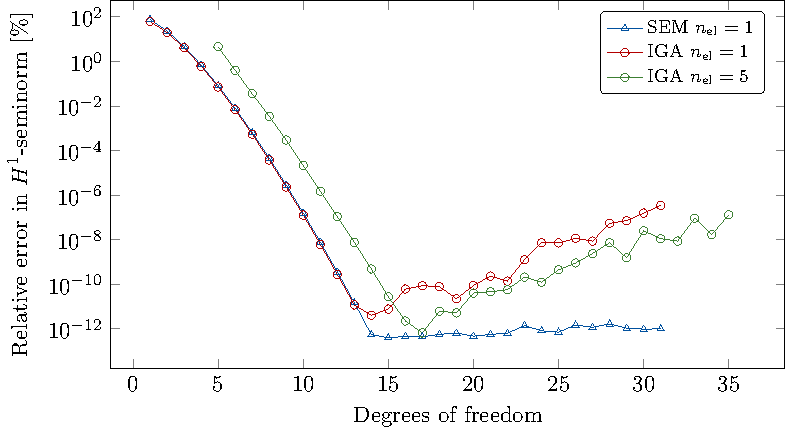
\includegraphics[scale=1]{../../LaTeX/createFigures/TikzFigures/articleSEM_PhD/poisson}
%	\includegraphics[scale=1]{Figure3}
	\caption{\textbf{Poisson 1D problem}: Illustration of the spectral convergence for SEM and IGA.}
	\label{Fig5:poisson}
\end{figure}
\begin{figure}
	\centering
	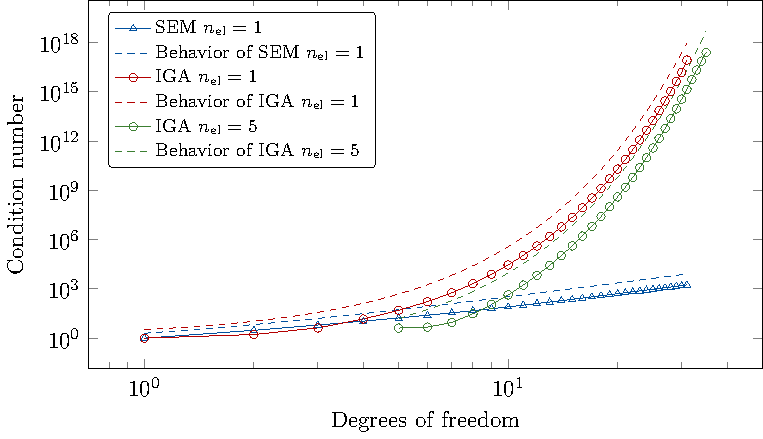
\includegraphics[scale=1]{../../LaTeX/createFigures/TikzFigures/articleSEM_PhD/poisson_cond}
%	\includegraphics[scale=1]{Figure3}
	\caption{\textbf{Poisson 1D problem}: An exponential behavior of the condition number is obtained for IGA, but only algebraic order is obtained for SEM when considering $\check{p}$-refinement and $\check{k}$-refinement, respectively. The behavior estimates for the two methods (found in \Cref{Eq5:condSEM,Eq5:condIGA2}, respectively) has been added}
	\label{Fig5:poisson_cond}
\end{figure}

\subsection{Rigid scattering on a sphere}
Consider the S1 benchmark problem in \cite{Venas2019e3s} where a unit sphere ($R_0=\SI{1}{m}$) is impinged by the plane wave in \Cref{Eq5:p_inc}. In the special case of $\vec{d}_{\mathrm{s}}=\vec{e}_{\mathrm{z}}$ the analytic solution to the problem is given by\footnote{Where $\besselj_n(x)$ is the $n^{\mathrm{th}}$ spherical Bessel function of the first kind and $\hankel_n(x)$ is the $n^{\mathrm{th}}$ spherical Hankel function of the first kind.} (expressed using spherical coordinates)
\begin{equation}\label{Eq5:analyticSolution}
	p(r,\theta) = -\legendre_{\mathrm{inc}}\sum_{n=0}^\infty \imag^n (2n+1) \frac{\besselj_n'(kR_0)}{\hankel_n'(kR_0)} \legendre_n(\cos\theta)\hankel_n(kr)
\end{equation}
which can be generalized to arbitrary vectors $\vec{d}_{\mathrm{s}}$ using a orthogonal transformation. In the S1 benchmark problem the incident plane wave travels in the direction
\begin{equation}
	\vec{d}_{\mathrm{s}} = -\begin{bmatrix}
		\cos\beta_{\mathrm{s}}\cos\alpha_{\mathrm{s}}\\
		\cos\beta_{\mathrm{s}}\sin\alpha_{\mathrm{s}}\\
		\sin\beta_{\mathrm{s}}
	\end{bmatrix}, \quad\text{where}\quad \alpha_{\mathrm{s}} = \ang{240},\,\beta_{\mathrm{s}} = \ang{30}.
\end{equation}
We shall use the same number of terms in the analytic series in \Cref{Eq5:analyticSolution} as the number of basis functions in the radial direction in the infinite elements to eliminate pollution from the infinite elements (cf. \cite{Gerdes1999otp}). In the experiments we choose the Bubnov--Galerkin unconjugated (BGU) formulation and we only use $N=3$ radial basis functions in the infinite elements to lower the conditioning of the system. The differences in the solutions are illustrated in \Cref{Fig5:Benchmarks_NearField}, where it is apparent that using only three terms in the series of the analytic solution is not even close to represent the full solution. But for the sake of convergence analysis it makes sense to consider this case to remove redundant noise from the infinite elements.
\begin{figure}
	\centering
	\begin{subfigure}[t]{0.48\textwidth}
		\centering
		%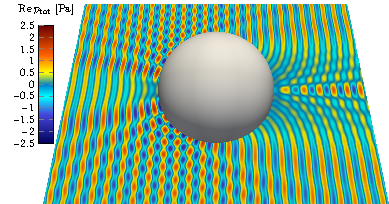
\includegraphics{../../LaTeX/createFigures/TikzFigures/articleJenserud/nearFields_S5_SHBC_real}
		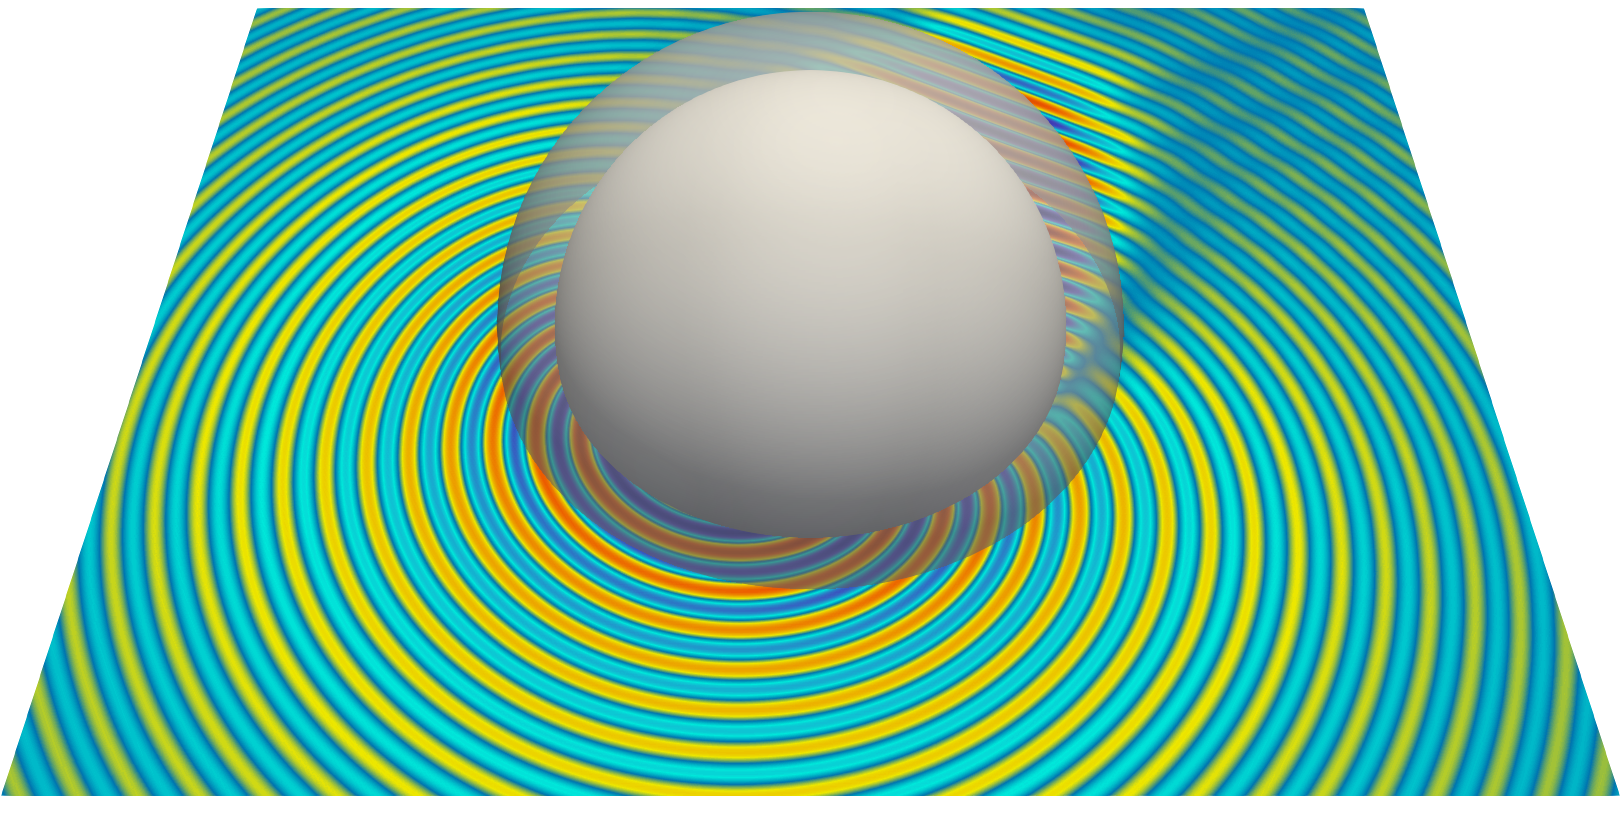
\includegraphics[width=\textwidth]{../../graphics/MA8502/Ninf}
		\label{Fig5:S1Ninf}
	\end{subfigure}
	~
	\begin{subfigure}[t]{0.48\textwidth}
		\centering
		%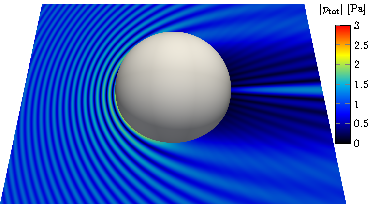
\includegraphics{../../LaTeX/createFigures/TikzFigures/articleJenserud/nearFields_S5_SHBC_abs}
		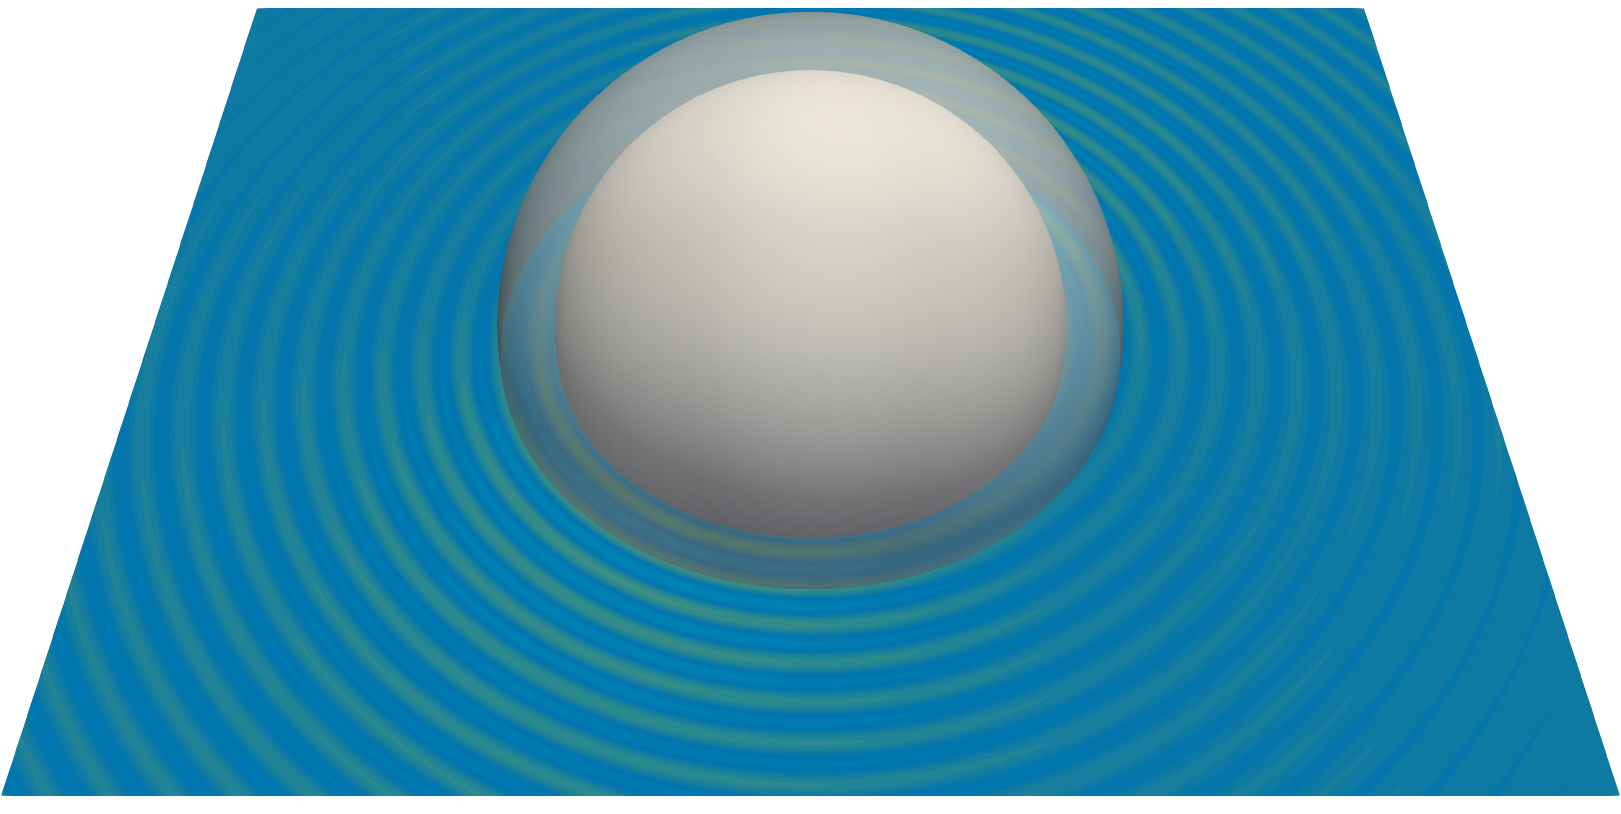
\includegraphics[width=\textwidth]{../../graphics/MA8502/N2}
		\label{Fig5:S1N2}
	\end{subfigure}
	\caption{\textbf{Rigid scattering on a sphere}: Plots of the near field of the scattered pressure resulting from a plane wave incident on a sphere at $f=\SI{10}{kHz}$. The plot to the left is the full solution, whereas the plot to the right is the solution resulting from the three first terms in the series expansion of the exact solution. The visualization was done in \href{http://www.paraview.org/}{Paraview}.}
	\label{Fig5:Benchmarks_NearField}
\end{figure}

%We use the following definition of the energy norm (as in \cite{Venas2018iao})
\begin{equation}\label{Eq5:energyNormFluids}
	\energyNorm{p}{\Omega_{\mathrm{a}}} = \sqrt{\int_{\Omega_{\mathrm{a}}} \left|\nabla p\right|^2 + k^2|p|^2 \idiff\Omega}
\end{equation}
and compute the integral by high order Gaussian quadrature (as the error should be more accurately computed than using the GLL nodes)
\begin{align*}
	\int_{\Omega_{\mathrm{a}}} \left|\nabla p\right|^2 + k^2|p|^2 \idiff\Omega &= \sum_{e=1}^{n_{\mathrm{el}}} \int_{\Omega_{\mathrm{a}}^e} \left|\nabla p\right|^2 + k^2|p|^2 \idiff\Omega\\
	&= \sum_{e=1}^{n_{\mathrm{el}}} \int_{-1}^1\int_{-1}^1\int_{-1}^1 \left(\left|\nabla p\right|^2 + k^2|p|^2\right)J \idiff\xi\idiff\eta\idiff\zeta.
\end{align*}
The meshes for both IGA and SEM are made based on 6 patches as illustrated in \Cref{Fig5:mesh}.
\begin{figure}
	\centering
	\begin{subfigure}[t]{0.4\textwidth}
		\centering
		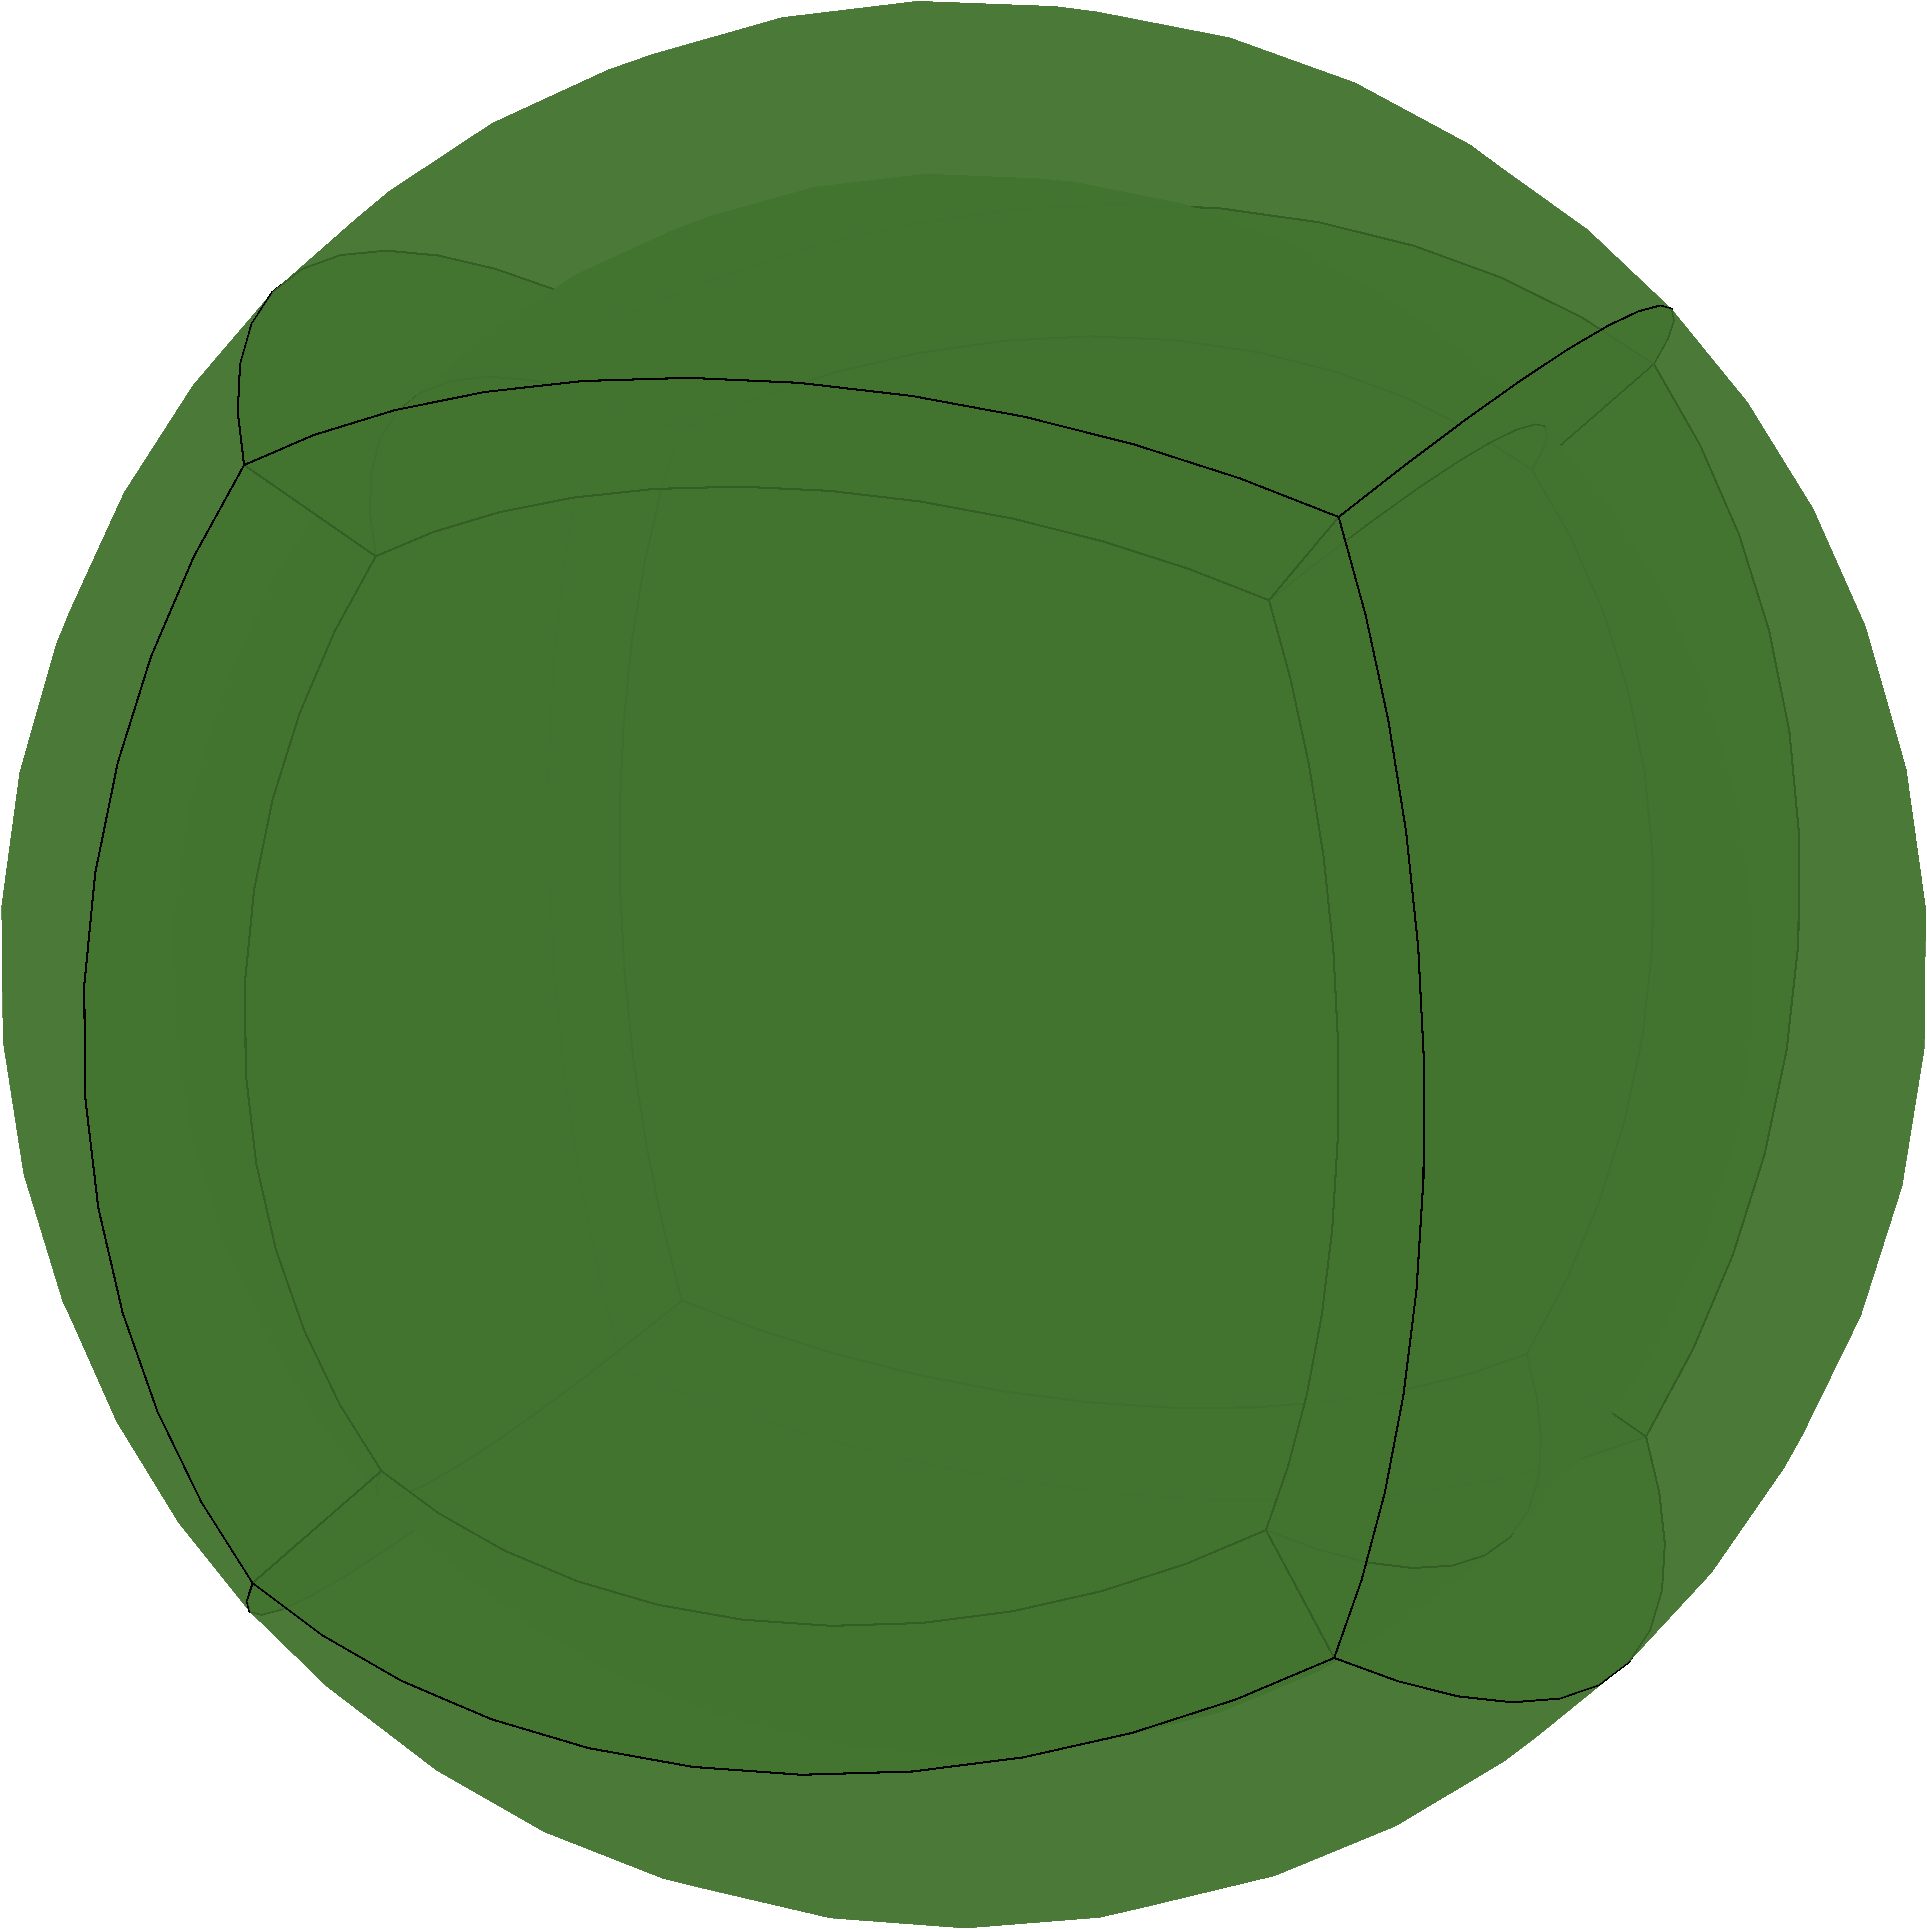
\includegraphics[width=\textwidth]{../../graphics/S1/S13D_IGA}
		\caption{IGA mesh}
	\end{subfigure}
	~    
	\begin{subfigure}[t]{0.4\textwidth}
		\centering
		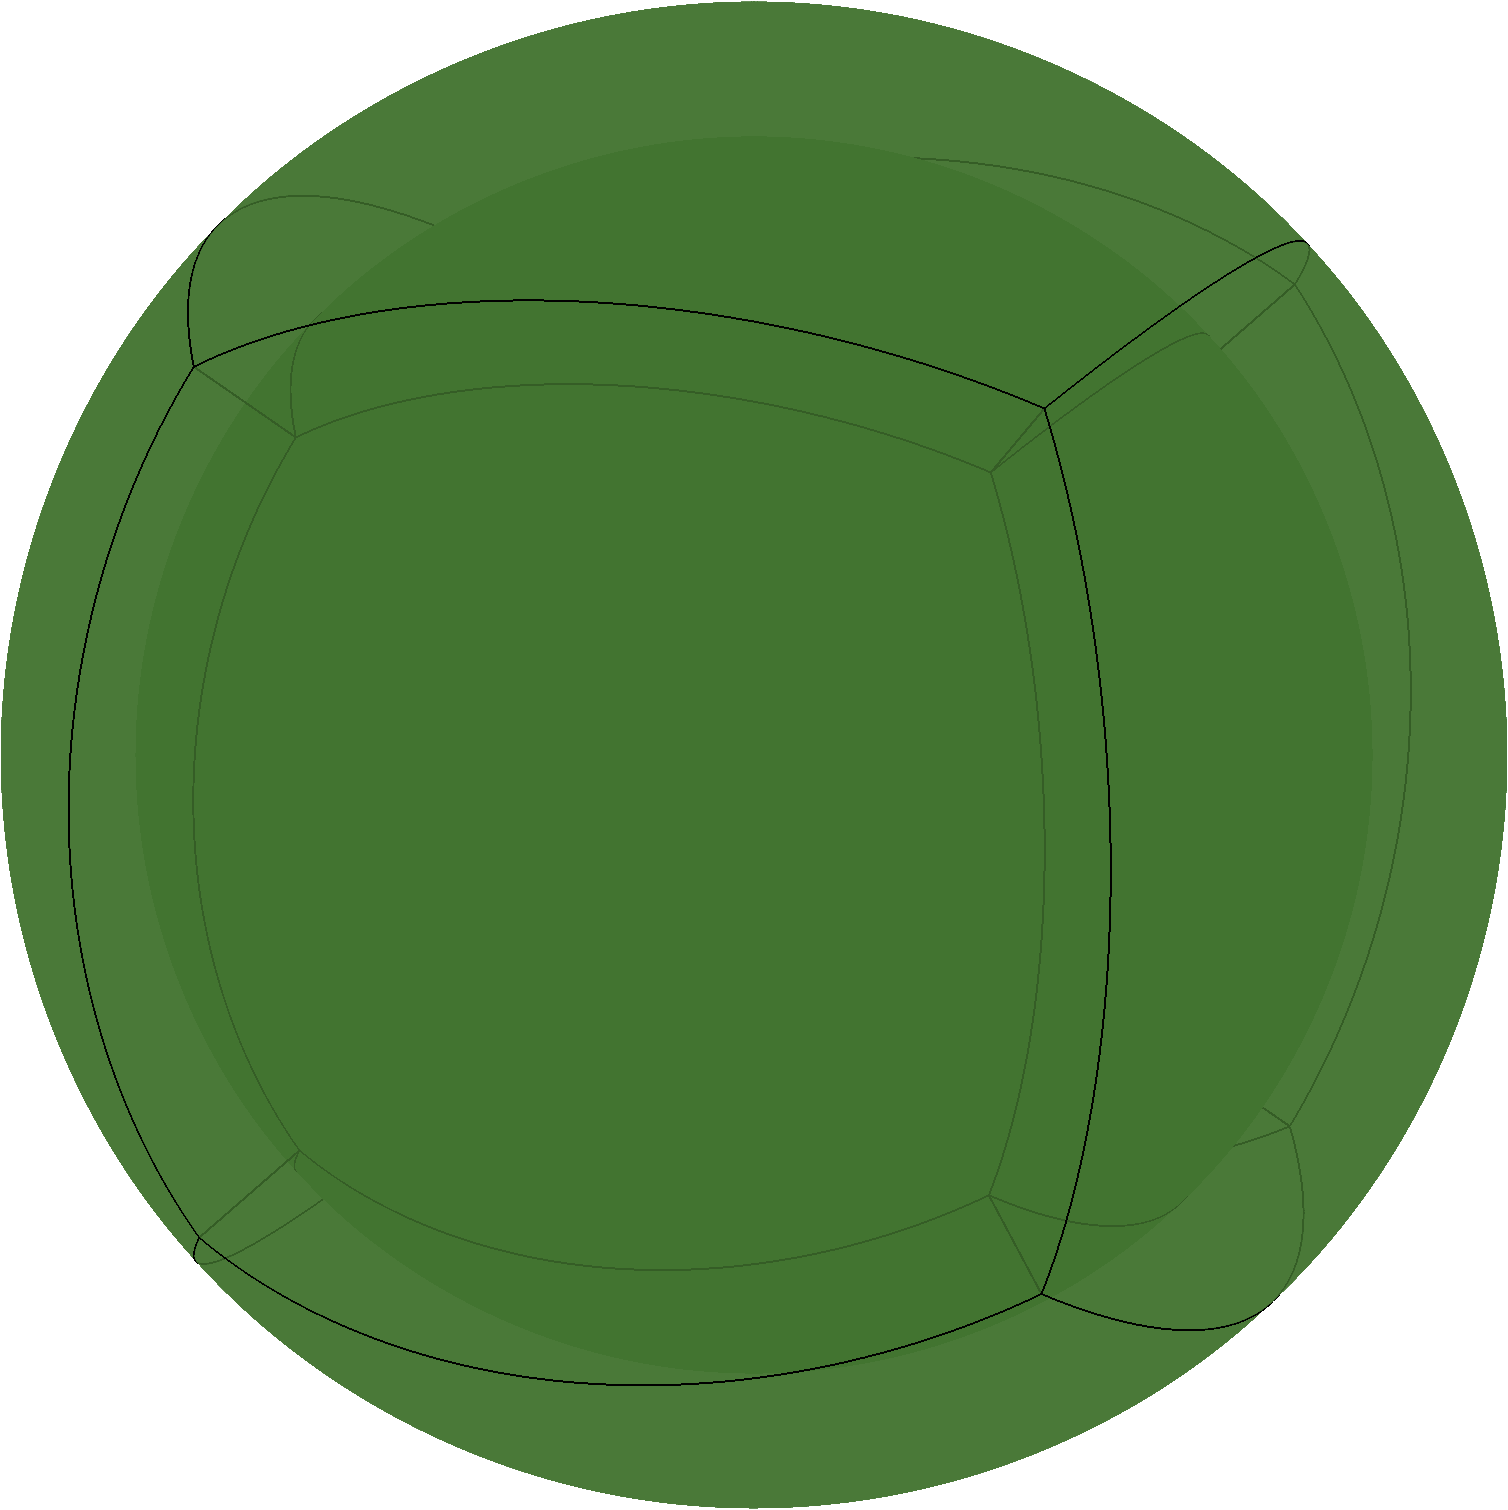
\includegraphics[width=\textwidth]{../../graphics/S1/S13D_SEM}
		\caption{SEM mesh}
	\end{subfigure}
	\caption{\textbf{Rigid scattering on a sphere}: The exact IGA meshing of the spherical shell domain is visually identical to the SEM approximation of the same geometry using only $\check{p}=4$.}
	\label{Fig5:mesh}
\end{figure}
In \Cref{Fig5:S1} we can again observe the expected spectral convergence for both IGA and SEM. Two simulations have been added for low and high frequencies\footnote{Given by $f=kc_{\mathrm{f}}/(2\PI)$ with $c_{\mathrm{f}}=\SI{1500}{m/s}$.}, $f=\SI{1}{kHz}$ and $f=\SI{10}{kHz}$, respectively. For the high frequency case, it is apparent that the geometry approximation is of less importance compared to the low frequency case as the error from resolving the wavelength is dominating the error in the geometry approximation. We can again here observe the instabilities for IGA for high polynomial orders.
\begin{figure}
	\centering
	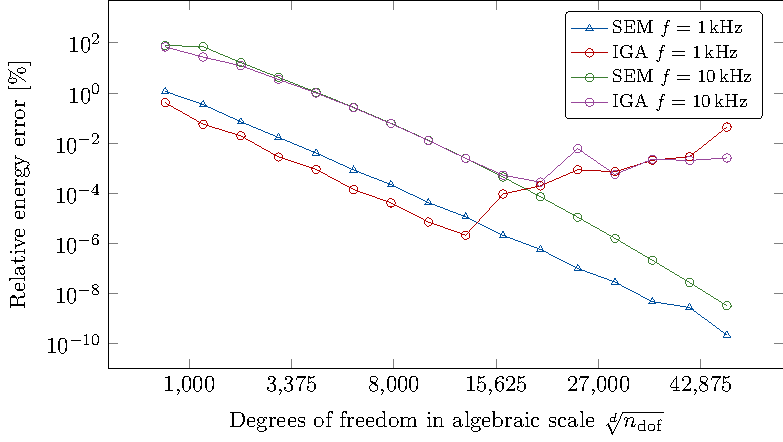
\includegraphics[scale=1]{../../LaTeX/createFigures/TikzFigures/articleSEM_PhD/S1}
%	\includegraphics[scale=1]{Figure3}
	\caption{\textbf{Rigid scattering on a sphere}: Illustration of the spectral convergence for SEM and IGA.}
	\label{Fig5:S1}
\end{figure}
This is again due to the large condition numbers in the stiffness and mass matrices for the IGA as illustrated in \Cref{Fig5:S1_cond}. 
\begin{figure}
	\centering
	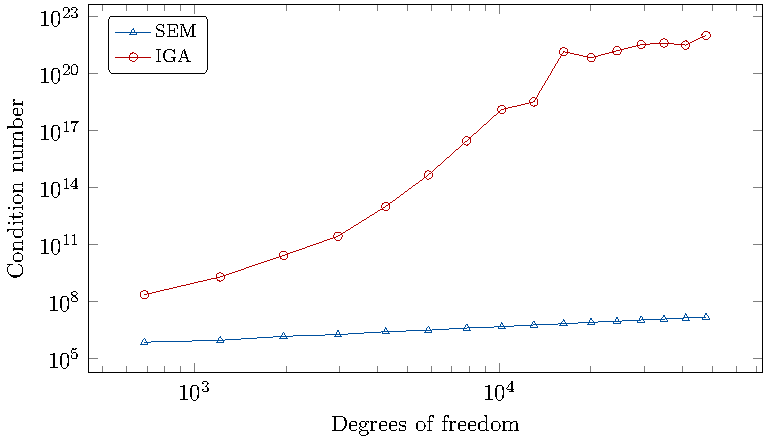
\includegraphics[scale=1]{../../LaTeX/createFigures/TikzFigures/articleSEM_PhD/S1_cond}
%	\includegraphics[scale=1]{Figure3}
	\caption{\textbf{Rigid scattering on a sphere}: An exponential behavior of the condition number is obtained for IGA, but only algebraic order is obtained for SEM when considering $\check{p}$-refinement. }
	\label{Fig5:S1_cond}
\end{figure}


The timings for building and solving the system for SEM and IGA are reported in \Cref{Fig5:S1_timeBuildSystem} and \Cref{Fig5:S1_timeSolveSystem}, respectively. These figures are added to show the total timings in \Cref{Fig5:S1_tot_time}. Here the key takeaway is the difference in convergence rate as a function of the time spent for both building and solving the system. The patch matrix construction is faster for SEM as the patch matrix sparsity goes as $\bigoh(n^{-1})$, which is in contrast to the corresponding IGA matrices which are fully dense. This is also the reason for better timings for solving the system using SEM as the global matrices are much sparser compared to the global matrices for IGA.
\begin{figure}
	\centering
	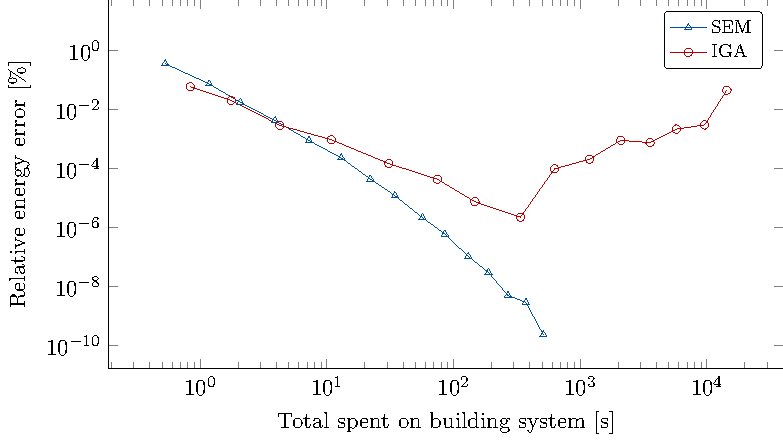
\includegraphics[scale=1]{../../LaTeX/createFigures/TikzFigures/articleSEM_PhD/S1_timeBuildSystem}
%	\includegraphics[scale=1]{Figure3}
	\caption{\textbf{Rigid scattering on a sphere}: The relative energy error is plotted against the total time spent on building the mass matrix, the stiffness matrix and the right-hand side vector.}
	\label{Fig5:S1_timeBuildSystem}
\end{figure}
\begin{figure}
	\centering
	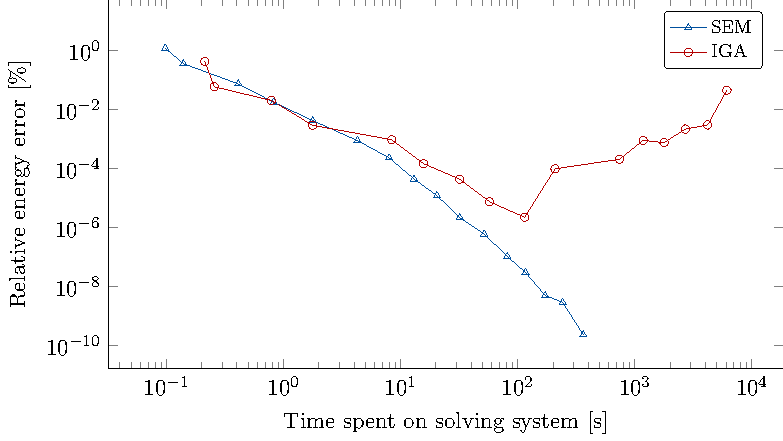
\includegraphics[scale=1]{../../LaTeX/createFigures/TikzFigures/articleSEM_PhD/S1_timeSolveSystem}
%	\includegraphics[scale=1]{Figure3}
	\caption{\textbf{Rigid scattering on a sphere}: The relative energy error is plotted against the computational time required to solve the system using a direct solver.}
	\label{Fig5:S1_timeSolveSystem}
\end{figure}
\begin{figure}
	\centering
	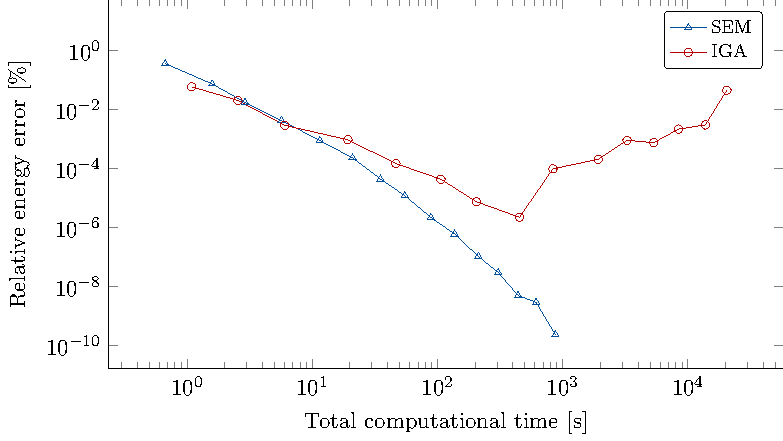
\includegraphics[scale=1]{../../LaTeX/createFigures/TikzFigures/articleSEM_PhD/S1_tot_time}
%	\includegraphics[scale=1]{Figure3}
	\caption{\textbf{Rigid scattering on a sphere}: The relative energy error is plotted against the total computational time (sum of the figures in \Cref{Fig5:S1_timeBuildSystem} and \Cref{Fig5:S1_timeSolveSystem}).}
	\label{Fig5:S1_tot_time}
\end{figure}

It should be mentioned that many improvements are here possible for both SEM and IGA. An iterative method (GMRES, BiCGstab, etc.) would be preferable for the SEM to reduce memory requirement and increase the computational efficiency. The tensor product structure in the IGA method could be exploited better instead of looping through every quadrature points individually~\cite{Antolin2015emc}.